\subsection{Electronics}

The electronics of the movement module were designed to support omnidirectional movement and basic obstacle detection. Our approach was to keep the system modular, efficient, and easy to assemble, using well-documented components compatible with Arduino-based development.

\subsubsection{Main Components and Setup}

\begin{itemize}
    \item \textbf{Microcontroller – ATmega328P}: Acts as the core of the movement module. It handles all the logic related to motor control, sensor reading, and decision-making. We used digital pins to interface with motor drivers and ultrasonic sensors.
    
    \item \textbf{DC Motors – JGB37-520 with encoders}: Three brushed DC motors are responsible for omnidirectional movement. Encoders are included for possible future use with closed-loop speed or distance control.
    
    \item \textbf{Motor Drivers – DRV8871}: Each motor is controlled through a dedicated DRV8871 H-bridge motor driver. These drivers are compact, reliable, and support the current required by the motors. Each driver is connected to the microcontroller via two control pins for speed and direction.
    
    \item \textbf{Omnidirectional Wheels – 58mm Nylon}: The wheels are attached to the motor shafts using 6mm aluminum hubs. These allow smooth and accurate multi-directional motion, essential for a patrol robot that must reposition itself easily.
    
    \item \textbf{Power Supply – LiPo battery with LM2596 regulator}: The circuit is powered by a LiPo battery. To provide consistent voltage to logic-level components and motor drivers, an LM2596 step-down regulator is used. It ensures the ATmega328P and sensors receive stable 5V output.
    
    \item \textbf{Obstacle Detection – HC-SR04 ultrasonic sensors}: Five ultrasonic sensors are distributed around the body of the robot to allow for basic obstacle detection. Each sensor is connected to a pair of digital pins on the ATmega328P, and they are intended to be triggered one at a time to avoid signal interference.
    
    \item \textbf{Wiring – Dupont cables and prototyping layout}: For prototyping, we used male-to-male and female-to-male Dupont jumper cables, enabling flexible reconfiguration and easy debugging during testing.
    
    \item \textbf{Camera module}: A compact camera module was added during the development phase to enable visual detection of the charging station via a QR code. This component provides the robot with basic computer vision capabilities, expanding its autonomy beyond obstacle-based navigation.
\end{itemize}

\subsubsection{System Relationship Overview}

\begin{figure}[H]
    \centering
    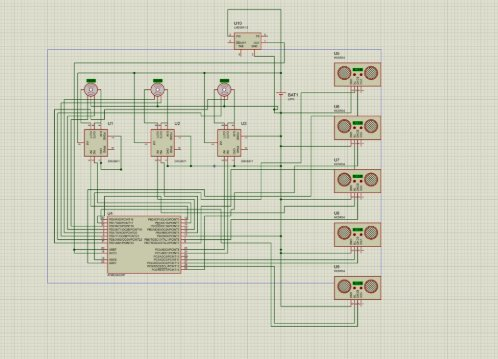
\includegraphics[width=0.7\linewidth]{../ReportMovementModule/images/Aspose.Words.728084da-df58-4b9d-a372-f65cffbdb23d.030.jpeg}
    \caption{Electronics System Diagram}
\end{figure}

\begin{itemize}
    \item The \textbf{ATmega328P} receives power from the regulated 5V supply.
    \item It sends PWM and direction signals to the \textbf{DRV8871 motor drivers}, which in turn control each of the \textbf{three motors}.
    \item The same microcontroller reads \textbf{ultrasonic distance values} from the HC-SR04 sensors.
    \item Based on sensor input and predefined logic, the microcontroller controls movement and reacts to obstacles through the actuation over the motors.
\end{itemize}

This configuration ensures the robot is capable of autonomous and reactive movement, with a clean base that allows for future integration of more advanced sensing and interaction features.
